\newpage
\section{Auswertung}
Die Werte der Bauteile des Schwingkreises sind:
\begin{align*}
    L&=\SI{16.78(09)}{\micro\henry}\\
    C&=\SI{2.066(006)}{\nano\farad}\\
    R_1&=\SI{67.2(2)}{\ohm}\\
    R_2&=\SI{682(1)}{\ohm}\\
\end{align*}

\subsection{Schwingungskurve}
\noindent
Aus der Schwingungskurve lässt sich mit Hilfe der Messwerte in der Tabelle \ref{tab:Uamp} eine einhüllende Funktion bestimmen. 
Dafür wird eine Fit-Funktion $U(t)$ bestimmt. Sie hat die Form:
\begin{equation}
    U(t)=A_0 \symup{e}^{-\mu t} \nonumber
\end{equation}
Da die Einhüllende an der x-Achse gespiegelt werden kann die Ausgleichsrechnung mit den Beträgen der Werte für 
$U_\text{Amp}$ durchgeführt werden. Die Konstanten bestimmen sich damit zu:
\begin{align*}
    A_0&=\SI{13.9205(2535)}{\V} & \mu&=(\num{1846.24473 \pm 58.380141 }) \mathrm{\frac{1}{s}} 
\end{align*}
Die Messwerte und der Fit ist in Abbildung \ref{img:huell} abgebildet.
\begin{figure}[H]
    \centering
    \includegraphics[width=0.7\textwidth]{build/plots/plot0.pdf}
    \caption{Die Messwerte der gedämpften Schwingung mit der einhüllenden Fit-Funktion.}
    \label{img:huell}
\end{figure}
\noindent
Mit diesen Werten lässt sich dann der der effektive Widerstand und die Abklingzeit des Schwingkreises bestimmen. 
Dafür werden die folgenden Gleichungen genutzt:
\begin{align*}
    R_\text{eff}&=\mu \cdot 4\pi L\\
    R_\text{eff}&= \SI{389.3060(124861)}{\ohm}  \\\\
    T_\text{ex}&=\frac{1}{2\pi\mu}\\
    T_\text{ex}&=\SI{86.2046838617(27258800232)}{\micro\second}
\end{align*}
Die Abweichung des genutzten Widerstandes von $R_\text{eff}$ beträgt:
\begin{equation}
    R_\text{eff}-R_1=\SI{322.1060(124877)}{\ohm} \nonumber
\end{equation}
Eine Abweichung von $\SI{50}{\ohm}$ wäre zu erwarten gewesen, da dies der Innenwiderstand des Generators ist.
Die tatsächliche Abweichung von $\approx \SI{300}{\ohm}$ könnte sich über ein Problem mit dem Generator erklären, welches erst bei späteren Messungen 
aufgefallen ist. Da diese Messung noch mit dem \enquote{defekten} Nadelimpulsgenerator durchgeführt wurde könnte er für die Abweichung verantwortlich sein.\\
Die nachfolgenden Rechnungen werden deshalb mit einem Widerstand von $R_1+\SI{50}{\ohm}$ durchgeführt.\\
In der folgenden Tabelle sind nochmal die Messwerte aufgetragen. 

\begin{table}[H]
    \centering
    \begin{tabular}{S [table-format=2.1] S [table-format=3.1]}
        \toprule
        {$U_\text{Amp} \mathbin{\scalebox{1.5} / }\si{\volt}$} & {$t_\text{Amp} \mathbin{\scalebox{1.5} / }\si{\micro\second}$}\\
        \midrule
        14.0 & 0.0 \\
        -11.5 & 14.0\\
        10.5 & 27.6\\
        -8.3 & 42.0\\
        7.8 & 54.00\\
        -6.0 & 68.0\\
        5.8 & 82.0\\
        -4.2 & 95.0\\
        4.1 & 108.0\\
        -3.0 & 122.0\\
        3.1 & 136.0\\
        -2.2 & 150.0\\
        2.5 & 163.0\\
        \bottomrule
    \end{tabular}
\caption{Die Messwerte der Amplitudenspannung mit ihren korrespondierenden Zeiten.}
\label{tab:Uamp}
\end{table}





\subsection{Aperiodischer Grenzfall}
\noindent
Die Messung zur Bestimmung des Widerstandes, bei dem der aperiodische Grenzfall eintritt, ergab:
\begin{equation}
    R_\text{ap}=\SI[]{1925}[]{\ohm} \nonumber
\end{equation}
Der theoretische Wert und die relative Abweichung von ihm, im Bezug auf den Theoriewert, berechnet sich dann zu:
\begin{align*}
    R_\text{ap theo}&= \sqrt{\frac{4L}{C}}=\SI{5699.8157(923168)}{\ohm}\\
    \frac{R_\text{ap theo}-R_\text{ap}}{R_\text{ap theo}}&=\SI{66.22698(54700)}{\percent}
\end{align*}
Die Abweichung der Werte lässt sich durch die in der Rechnung nicht beachteten Widerstände der anderen Bauteile erklären. 
Allerdings kann damit keine Abweichung dieser Größe erklärt werden. Dafür kann also wieder der Generator Verantwortlich gemacht werden.


\subsection{Resonanzüberhöhung}
Im folgenden wird die Resonanzüberhöhung untersucht. 
Die Messwerte der mit der angelegten Spannung normierten Kondensatorspannung und ihrer korrespondierenden Frequenzen finden sich in Tabelle \ref{tab:Uu0}.\\
Aus diesen Messwerten lässt sich der theoretische Faktor für die Resonanzüberhöhung $q_\text{theo}$ bestimmen.
Die experimentelle Resonanzüberhöhung lässt sich durch das Ablesen des Maximums aus den Messwerten bestimmen. \\
Dies entspricht dem Wert $q_\text{exp}=3.8$.\\
$q_\text{theo}$ berechnet sich über die folgenden Gleichungen, wobei $R$ dem Gesamtdämpfungswiderstand entspricht.
\begin{align*}
    q_\text{theo}&= \frac{1}{\omega_0RC}& \omega_0&=\sqrt{\frac{1}{LC}}\\
    \implies q_\text{theo}&=\sqrt{\frac{L}{R^2C}}=\SI{24.3(4)}{}
\end{align*}
Dies führt zu einer relativen Abweichung des experimentellen vom theoretischen Wert von $\SI{84.37(25)}{\percent}$.\\
In der folgenden Abbildung sind die Messwerte halblogarithmisch aufgetragen.
\begin{figure}[H]
    \centering
    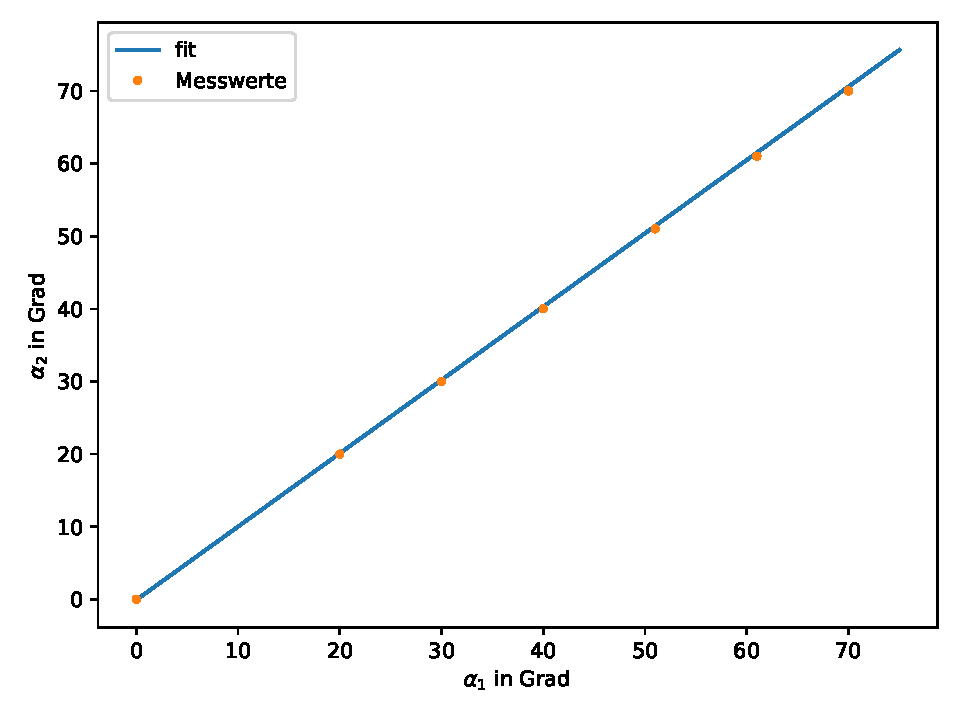
\includegraphics[width=0.7\textwidth]{build/plots/plot1.pdf}
    \caption{Die Messwerte zur Resonanzüberhöhung halblogarithmisch dargestellt.}
    \label{img:Uu0}
\end{figure}
\noindent
Für die Bestimmung der experimentellen Halbwertsbreite werden die Messwerte um den Peak mit einer quadratischen Funktion angenähert und die x-Werte
bei den Spannungswerten $\frac{{\left(\frac{U}{\symup{U_0}}\right)}_\text{max}}{\sqrt{2}}$ bestimmt. Dies wird in der Abbildung \ref{img:quad} noch einmal veranschaulicht.
Dort sind die Messwerte des relevanten Wertebereiches, inklusive aller zuvor erwähnten Funktionen, linear dargestellt.
Außerdem sind die Schnittgerade bei $\frac{{\left(\frac{U}{\symup{U_0}}\right)}_\text{max}}{\sqrt{2}}$ und die quadratische Fit-Funktion eingezeichnet.\\
Der Fit besitzt dabei die Form:
\begin{equation*}
    f(x)= A\cdot x^2 +B\cdot x+ C
\end{equation*}
mit 
\begin{table}[H]
    \centering
    \sisetup{table-format=1.3}
    \begin{tabular}{ S | S [table-format=2.5] @{$ \pm{}$} S [table-format=4.5] S[table-format=1.1] }
        \toprule
        {Parameter} & \multicolumn{3}{c}{ Bestimmte Werte} \\
        \midrule
        \text{A}	& \num{-8.3}\SI{1e-8}{}& \num{0.5}\SI{1e-8}{}&\si{\second\squared} \\
        \text{B}	&\num{0.00432}  & \num{0.00028}&\si{\second}  \\
        \text{C}	&\num{-52}  & \num{4} &\\
        \bottomrule
    \end{tabular}
\caption {Berechnete Werte für die quadratische Fit-Funktion gerundet auf die fünfte Nachkommastelle.}
\label{tab:quad}
\end{table}


\noindent
Die Schnittpukte mit der Schnittgeraden lassen sich über gleichsetzten und auflösen mit der p,q-Formel bestimmen.\\
Mit diesen Werten lässt sich dann die expmerimentelle Halbwertsbreite 
\begin{align*}
    \omega_\text{1,2}&=-\frac{B}{2A} \pm \sqrt{\frac{B^2}{4A^2}-\frac{C}{A}}\\
    \omega_\text{1}&=\SI{22395.6 }{\hertz} & \omega_\text{2}&=\SI{29532.0 }{\hertz} \\
    (\nu_+ -\nu_-)_\text{exp} &= \omega_1-\omega_2 =\SI{7.1364}{\kilo\hertz}
\end{align*}
Eingezeichnet sind diese Werte noch einmal in der folgenden Abbildung.


\begin{figure}[H]
    \centering
    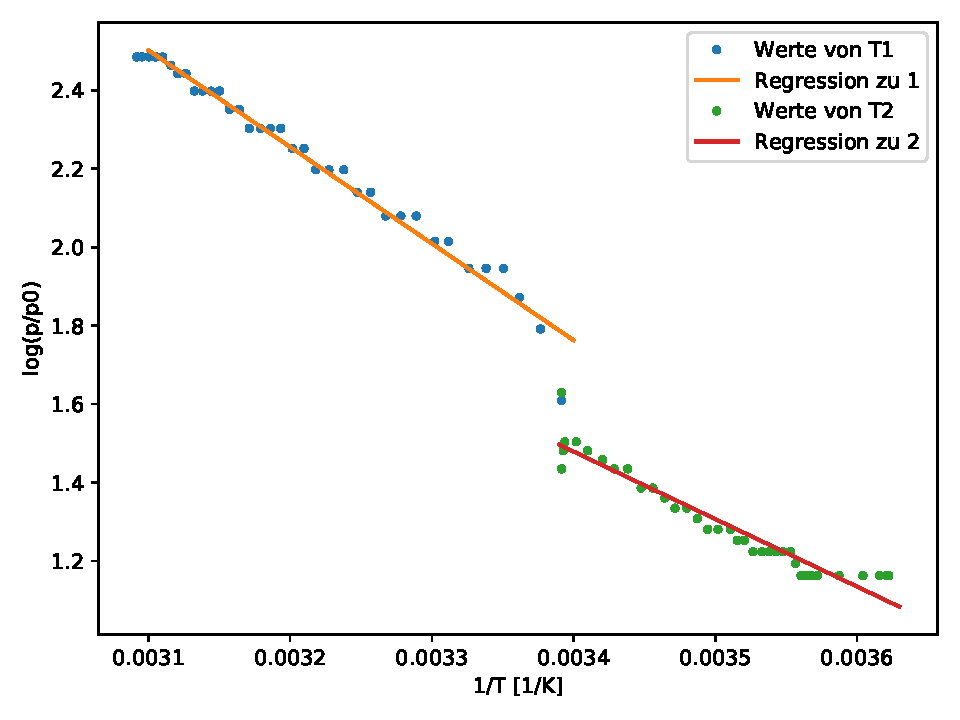
\includegraphics[width=0.9\textwidth]{build/plots/plot2.pdf}
    \caption{Die Messwerte zur Resonanzüberhöhung linear dargestellt. Zusätzlich ist noch die Fit-Funktion, die experimentelle Halbwertsbreite und die Schnittgerade abgebildet. }
    \label{img:quad}
\end{figure}

\noindent
Die theoretische Halbwertsbreite berechnet sich mit der folgenden Formel:
\begin{align*}
    (\nu_+ -\nu_-)_\text{theo} &\approx \frac{R}{L}\\
    \implies (\nu_+ -\nu_-)_\text{theo} &\approx \SI{6.98(04)}{\kilo\hertz}
    \intertext{Dies führt zu einer relativen Abweichung vom Theoriewert von:}
    \frac{(\nu_+ -\nu_-)_\text{exp} -(\nu_+ -\nu_-)_\text{theo}} { (\nu_+ -\nu_-)_\text{theo} }&= \SI{2.2(6)}{\percent}
\end{align*}

\noindent
In der folgenden Tabelle finden sich dann nochmal die Messwerte der normierten Kondenstatorspannung und der dazugehörigen Frequenzen.
\begin{table}[H]
    \centering
    \begin{tabular}{S [table-format=1.2] S [table-format=2.0]}
        \toprule
        {$\frac{U}{\symup{U_0}}$} & {$f \mathbin{\scalebox{1.5} / } \si{\kilo\hertz}$}\\
        \midrule
        1.08 & 5\\
        1.24 & 10\\
        1.44 & 15\\
        2.16 & 20\\
        2.40 & 21\\
        3.00 & 23\\
        3.40 & 24\\
        3.72 & 25\\
        3.80 & 26\\
        3.64 & 27\\
        3.12 & 28\\
        2.44 & 30\\
        1.60 & 33\\
        1.24 & 35\\
        0.84 & 40\\
        0.60 & 45\\
        0.44 & 50\\
        \bottomrule
    \end{tabular}
\caption{Die Messwerte Spannung im Verhältnis zur angelegten Spannung und die dazugehörigen Frequenzen.}
\label{tab:Uu0}
\end{table}






\subsection{Phasenverschiebung}
Die Messwerte zur Bestimmung der Phasenverschiebung zwischen der Erregerspannung und der Kondenstatorspannung sind in Tabelle \ref{tab:phi} aufgetragen.\\
Dabei wurde die Zeit $\increment t$ mit der Formel $\increment \phi =\increment t \cdot f \cdot 2\pi$ in einen Winkel umgerechnet.\\

\begin{table}[H]
    \centering
    \begin{tabular}{S [table-format=2.1] S [table-format=2.1] S [table-format=1.3]}
        \toprule
        {$f \mathbin{\scalebox{1.5} / } \si{\kilo\hertz}$} & {$\increment t \mathbin{\scalebox{1.5} / } \si{\micro\second}$} & {$\phi \mathbin{\scalebox{1.5} / } \si{\radian}$}\\
        \midrule
        5.0& 0.0 & 0.000  \\
        10.0 & 1.0 & 0.063 \\
        12.0 & 1.5 & 0.113 \\
        14.0 & 1.5 & 0.132 \\
        20.0 & 0.0 & 0.000 \\
        25.0 & 0.5 & 0.079 \\
        30.0 & 1.0 & 0.188 \\
        35.0 & 1.5 & 0.330 \\
        35.7 & 3.0 & 0.674 \\
        36.2 & 4.0 & 0.911 \\
        36.7 & 6.0 & 1.385 \\
        37.5 & 8.0 & 1.885 \\
        38.0 & 10.0 & 2.388\\
        38.2 & 11.0 & 2.644\\
        38.7 & 11.0 & 2.678\\
        40.0 & 11.0 & 2.765\\
        42.5 & 11.5 & 3.071\\
        45.0 & 11.0 & 3.110\\
        \bottomrule
    \end{tabular}
\caption{Die Messwerte der Phasenverschiebung zwischen Kondensator- und Erregerspannung bei unterschiedlichen Frequenzen. $\increment t$ ist dabei die Zeitdifferenz zwishen zwei Amplituden und $\phi$ diese umgewandelt in einen Winkel.}
\label{tab:phi}
\end{table}
\noindent
Grafisch dargestellt finden sich die Messwerte in der Abbildung \ref{img:plot3}. Dabei zeigt sich, dass für niedrige Frequenzen, bis auf eine kleine auftretende aber direkt wieder abflachende
Phasenverschiebung, keine Verschiebung auftritt.\\
Erst für Frequenzen ab $\SI{20}{\kilo\hertz}$ tritt eine wesentliche Phasenverschiebung zwischen den beiden Spannungen auf. \\
Diese steigt bis zu einer Frequenz von $\SI{40}{\kilo\hertz}$, wo sie dann konstant bei einem Wert von $\pi$ bleibt.
\begin{figure}[H]
    \centering
    \includegraphics[width=0.7\textwidth]{build/plots/plot3.pdf}
    \caption{Die Messwerte zur Phasenverschiebung halblogarithmisch dargestellt.}
    \label{img:plot3}
\end{figure}

\noindent
Diese Form ließe sich durch eine $arctan()$-Funktion beschreiben. Allerdings kann das ganze auch besser mit einer Sigmoids-Funktion bewerkstelligt werde, da diese 
gar keinen Schnittpunkt mit der x-Achse besitzt und ansonsten eine sehr ähnliche Form hat.\\
Mathematisch besitzt sie die Form:
\begin{equation}
    \phi(t)=\frac{A}{ 1 + \exp({-(x - B)/D))} }+ C
    \label{eqn:sig}
\end{equation}
Wenn nun der Bereich um die starke Steigung linear dargestellt wird, lässt sich auf ihm die Sigmoids-Funktion fitten. Dies führt zu den Funktionswerten:
\begin{table}[H]
    \centering
    \sisetup{table-format=1.3}
    \begin{tabular}{ S | S [table-format=5.5] @{$ \pm{}$} S [table-format=2.5] S }
        \toprule
        {Parameter} & \multicolumn{3}{c}{ Bestimmte Werte} \\
        \midrule
        \text{A}	&\num{2.94167}  & \num{0.08634} & \; \si{\radian}\\
        \text{B}	&\num{36988.06355}  & \num{84.81132} & \\
        \text{C}	&\num{0.08872}  & \num{0.05578} & \; \si{\radian}\\
        \text{D}	&\num{838.78531}  & \num{67.35911} & \\
        \bottomrule
    \end{tabular}
\caption {Berechnete Werte für die Sigmoids-Funktion gerundet auf die fünfte Nachkommastelle.}
\label{tab:sigmoid}
\end{table}
\noindent
Eingezeichnet wird dies in der Abbildung \ref{img:plot4}. Dort sind auch noch die Schnittgeraden der charakteristischen Punkte $w_1$, $w_2$ und $w_\text{res}$ dargestellt.\\
An diesen Punkten hat die Sigmoids-Funktion die Werte $\frac{\pi}{4}$, $\frac{3\pi}{4}$ und $\frac{\pi}{2}$.\\
Berechnet werden die Schnittpunkte über das umstellen der Funktion \refeq{eqn:sig} nach x.
\begin{equation*}
    x=(-D\cdot\ln{(A/(\phi-C)-1)+B}
\end{equation*}
Die Ergebnisse dieser Rechnung sind, zusammen mit den später berechneten theorestischen Werten, in \ref{tab:omegas} aufgetragen.

\begin{figure}[H]
    \centering
    \includegraphics[width=0.85\textwidth]{build/plots/plot4.pdf}
    \caption{Eine lineare Darstellung der Messwerte umd die charakteristischen Punkte, wobei die Sigmoids-Funktion und die charakteristischen Punkte auch dargestellt werden.}
    \label{img:plot4}
\end{figure}

\noindent
Die theoretischen Werte für die drei Frequenzen lassen sich mit den folgenden zwei Formeln bestimmen.\\
Dabei ist $R$ wieder der Gesamtwiderstand.
\begin{align*}
    w_\text{1,2 theo}&= \pm \frac{R}{2L} + \sqrt{\frac{R^2}{4L^2}+\frac{1}{LC}}\\
    W_\text{res theo}&= \sqrt{\frac{1}{LC}-\frac{R^2}{4L^2}}
\end{align*}
Die Ergebnisse dieser Rechnung finden sich,wie zuvor erwähnt, in der folgenden Tabelle wieder.

\begin{table}[H]
    \centering
    \sisetup{table-format=1.3}
    \begin{tabular}{ S | S [table-format=2.2] @{$ \quad \pm{}$} S [table-format=1.2] S [table-format=2.2]  S [table-format=2.2] @{$ \quad \pm{}$} S [table-format=1.2] }
        \toprule
        \multicolumn{1}{c|}{Frequenz} & \multicolumn{2}{p{4cm}}{\centering Theoretischer Wert \\$ \si{\kilo\hertz}$} & 
        \multicolumn{1}{p{4cm}}{\centering Experimenteller Wert\\ $ \si{\kilo\hertz}$} & 
        \multicolumn{2}{p{4cm}}{\centering Abweichung von der Theorie \\ $\si{\percent}$} \\
        \midrule \cmidrule(lr){2-3}\cmidrule(lr){5-6}
        $w_\text{res}$   &\num{16.98} & \num{0.28}       &\num{3.70}       &\num{78.20} &\num{0.35}\\
        $w_\text{1}	$    &\num{17.34} & \num{0.28}       &\num{3.60}       &\num{79.23}&\num{0.33}\\
        $w_\text{2}$	 &\num{16.64} & \num{0.27}       &\num{3.80}       &\num{77.2}&\num{0.40}\\
        \bottomrule
    \end{tabular}
\caption {Vergleich der charakteristischen Frequenzen. \newline Dabei ist $w_\text{res}$ die für den Wert $\frac{\pi}{2}$, 
$w_\text{1} $ für $\frac{\pi}{4}$ und $w_\text{2} $ für $\frac{3 \pi}{4}$.}
\label{tab:omegas}
\end{table}

\noindent
Auch hier weichen die experimentellen Werte wieder sehr stark von den theoretischen ab. Da für diese Messung ein neuer, voll funktionstüchtiger Nadelimpulsgenerator zur Verfügung gestellt
wurde kann dieser nicht wieder als Grund für starke Abweichungen genannt werden.\\

